\documentclass{article}
\usepackage[utf8]{inputenc}
\usepackage{graphicx}
\usepackage{hyperref}
\usepackage{listings}
\setlength{\oddsidemargin}{0in}
\setlength{\evensidemargin}{0in}
\setlength{\textheight}{9in}
\setlength{\textwidth}{6.5in}
\setlength{\topmargin}{-0.5in}

\title{122B Spring 2016 \\ Program 2}
\author{Russell Miller and Rylan Schaeffer }

\begin{document}

\maketitle

\section*{Introduction}
\indent \indent Quicksort, Quickselect and Deterministicselect are three algorithms that can be used to select the $k$th smallest element of an unordered list. We compared their relative performance (measured by time to correct result) as a function of the length of the list. To do so, we analyzed the algorithms and gathered experimental data from randomly generated lists to confirm our analysis. We conclude that although the performances of the three algoriths are comparable for shorter lists, the performances begin to differ for longer lists, with quickselect emerging as the clear winner.

\section*{Algorithm Analysis and Pseudocode}
\subsection*{Quickselect}
\indent \indent 



\subsection*{Deterministicselect}
\indent \indent 


\subsection*{Quicksort}
\indent \indent Quicksort differs from the two prior algorithms in that quicksort is a sorting algorithm; that is, quicksort rearranges the list in increasing order. To select the $kth$ smallest element, one simply selects the $k$th element from the sorted list.

Quicksort sorts the list using the same principle that Quickselect uses: an element is selected from the list (called the pivot), and then the list is partitioned into two lists such that all elements in one list are less than the pivot and all elements in the other list are greater than the pivot. But rather than recursing into one of the two new lists as Quickselect does, Quicksort applies the same sorting procedure recursively to both lists. Thus, Quicksort performs comparatively more work than Quickselect.

\subsection*{Pseudocode}
See section Pseudocode on the last two pages for psuedocode of all three algorithms.

\pagebreak

\section*{Empirical Study}
\indent \indent To investigate the relative performance of the three algorithms, we generated 1000 lists: 200 containing $10^2$ integers between one and one million, 200 containing $10^3$ integers between one and one million, 200 containing $10^4$ integers between one and one million, 200 containing $10^5$ integers between one and one million, and 200 containing $10^6$ integers between one and one million.

For each list, we generated a random number $k$ between one and the length of the list, and then timed how long each of the three algorithm took to select the $k$th element from the list. The results were saved to a comma separated values (CSV) file for subsequent analysis. Below are the first few lines of our collected data.

\bigskip

\begin{tabular}{|r|r|r|r|r|r|}
\hline
Sample Number	& listLength & kvalue &	quickselect (s)	& quicksort (s) & deterministicselect (s)\\
\hline
1	& 100	& 57	& 0.035	& 0.026	& 0.033\\
2	& 100	& 51	& 0.032	& 0.036	& 0.036\\
3	& 100	& 23	& 0.028	& 0.032	& 0.033\\
4	& 100	& 58	& 0.025	& 0.034	& 0.031\\
5	& 100	& 1	& 0.034	& 0.028	&0.031\\
\hline
\end{tabular}

\bigskip

\indent \indent The three algorithms were implemented in Python 2.7 - see files quickselect.py, quicksort.py and deterministicselect.py. A fourth Python 2.7 script was written to generate lists of random numbers of a specified length - see randGen.py. Bash scripting was used to run randGen.py and feed its output to each algorithm, and then write each algorithm's time to the CSV file - see pipeline.sh. To generate your own dataset, run ``./pipeline.sh" from the command line with the four Python scripts in the same directory as the pipeline.sh script.

\section*{Results}

\indent \indent We began our analysis by plotting the time to correct result as measured in seconds against the list length as measured by number of integers.

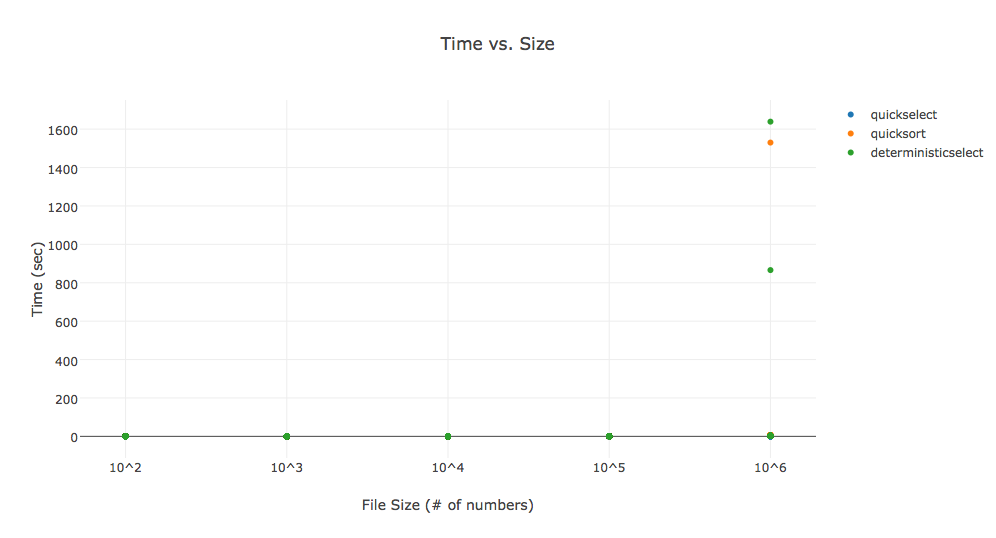
\includegraphics[scale=0.45]{resultsWoutliers}

Three outliers, two from deterministicselect and one from quicksort, clearly skewed our plot. We examined the lists that took substantially longer to complete to determine why; we discovered Russell's computer had shifted into sleep mode and resumed executing once awoken. We felt justified in excluding the outliers and recreated the previous plot to gain a better sense of each algorithm's performance.

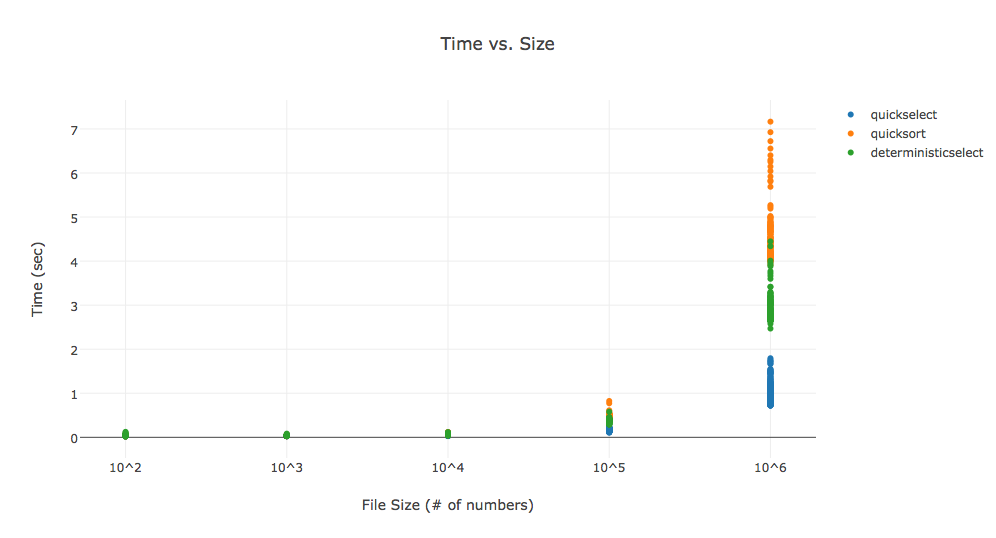
\includegraphics[scale=.45]{results}

To compare performance by list length, we plotted the performance of all three algorithms in a histogram for each of the five list lengths ($10^2, 10^3, 10^4, 10^5, 10^6$, respectively).

\section*{Future Directions}
multiple selects for same list - quicksort faster?\\

at which point one algorithm surpasses the other?\\

exactly what is the ratio of performance between algorithms?

\section*{Conclusion}

\section*{Citations}
Quicksort. Wikipedia. Accessed June 6th, 2016. \url{https://en.wikipedia.org/wiki/Quicksort}\\

\noindent Quickselect. Wikipedia. Accessed June 6th, 2016. \url{https://en.wikipedia.org/wiki/Quickselect}\\

\noindent Median of Medians. Wikipedia. Accessed June 6th, 2016. \url{https://en.wikipedia.org/wiki/Median_of_medians}

\pagebreak

\section*{Pseudocode}

\subsection*{Quickselect Pseudocode}
Copied from Wikipedia article on Quickselect (see Citations):
\begin{lstlisting}
function quickselect(A, lo, hi)
    if lo < hi then
        p := partition(A, lo, hi)
        quicksort(A, lo, p)
        quicksort(A, p + 1, hi)
        
function partition(list, left, right, pivotIndex)
     pivotValue := list[pivotIndex]
     swap list[pivotIndex] and list[right]
     storeIndex := left
     for i from left to right-1
         if list[i] < pivotValue
             swap list[storeIndex] and list[i]
             increment storeIndex
     swap list[right] and list[storeIndex]
     return storeIndex
     
function select(list, left, right, n)
     loop
         if left = right
             return list[left]
         pivotIndex := (left + right) / 2
         pivotIndex := partition(list, left, right, pivotIndex)
         if n = pivotIndex
             return list[n]
         else if n < pivotIndex
             right := pivotIndex - 1
         else
             left := pivotIndex + 1
\end{lstlisting}

\subsection*{Deterministicselect Pseudocode}
Adapted from Wikipedia article on Median Of Medians (see Citations):

\begin{lstlisting}
function deterministicselect(list, left, right, n)
    loop
        if left = right
             return left
        pivotIndex := pivot(list, left, right)
        pivotIndex := partition(list, left, right, pivotIndex)
        if n = pivotIndex
            return n
        else if n < pivotIndex
            right := pivotIndex - 1
        else
            left := pivotIndex + 1
            
function partition(list, left, right, pivotIndex)
     pivotValue := list[pivotIndex]
     swap list[pivotIndex] and list[right]
     for i from left to right-1
         if list[i] < pivotValue
             swap list[storeIndex] and list[i]
             increment storeIndex
     swap list[right] and list[storeIndex]
     return storeIndex
     
function pivot(list, left, right)
     if right - left < 5:
         return partition5(list, left, right)
     for i from left to right in steps of 5
         subRight := i + 4
         if subRight > right:
             subRight := right

         median5 := partition5(list, i, subRight)
         swap list[median5] and list[left + floor((i - left)/5)]
     newRight = left + ceil((right - left) / 5) - 1
     newK = left + (right - left)/10
     return select(list, left, newRight, newK)
     
function partition5(list, left, right)
     return left + index of median of list[left:right]
\end{lstlisting}


\subsection*{Quicksort Pseudocode}
Copied from Wikipedia article on Quicksort (see Citations):

\begin{lstlisting}
function quicksort(A, lo, hi)
    if lo < hi then
        p := partition(A, lo, hi)
        quicksort(A, lo, p)
        quicksort(A, p + 1, hi)

function partition(A, lo, hi)
    pivot := A[lo]
    i := lo - 1
    j := hi + 1
    loop forever
        do
            i := i + 1
        while A[i] < pivot
        do
            j := j - 1
        while A[j] > pivot
        if i >= j then
            return j
        swap A[i] with A[j]
\end{lstlisting}

\end{document}
